\documentclass[11pt]{article}
\usepackage[utf8]{inputenc}

\usepackage{geometry}
\geometry{a4paper}

\usepackage{graphicx}
\usepackage{hyperref}
\usepackage[parfill]{parskip}
\usepackage{amsmath, amssymb}
\usepackage{fdsymbol}
\usepackage{color,soul}

% remove section numbering
\makeatletter
\renewcommand{\@seccntformat}[1]{}
\makeatother

% make subsubsection italic
\usepackage{sectsty}
\subsubsectionfont{\itshape}

\renewcommand{\arraystretch}{1.4}

\title{Probability Theory \& Statistics}
\date{}
\author{}

\begin{document}
\maketitle
\clearpage

\section{Conditional Probability}

\subsection{Introduction}

All probabilities are conditional probabilities 
-- there is always some prior knowledge (or assumption) built 
into every probability. 
Heads or tails coin flips assumes a fair coin, 
choosing a marble from an bag assumes the marbles are indistinguishable.
Equivalently, 
conditional probabilities \emph{are probabilities}, 
the same properties and axioms apply to conditional probabilities that apply
to unconditional probabilities.%
\footnote{We won't prove this, but feel free to try!}

Beyond prior or assumed knowledge, 
conditioning allows us to further update probabilities 
or beliefs given new evidence (or given evidence we wished we had). 
For example, 
suppose \(R\) is the event it will rain, 
and \(P(R)\) is the probability it will rain. 
If we observe a change in the weather, 
maybe dark clouds appear in the sky, 
the probability it will rain is expected to increase,
i.e., \(P(R) < P(R|C)\).%
\footnote{We observe something, 
obtain some new information, 
or speculate about what information we might get!}

\begin{figure}[h!]
\centering
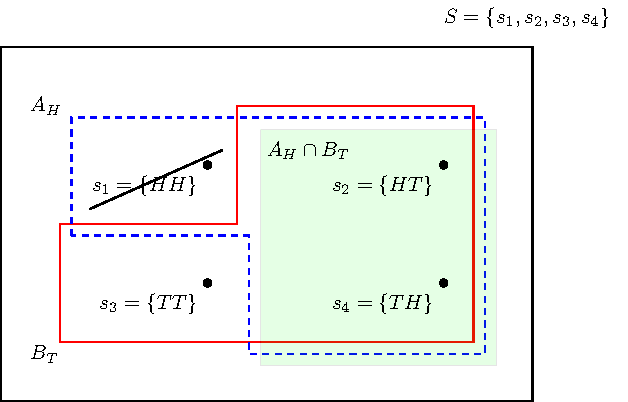
\includegraphics[width=0.75\linewidth]{tikz/figure1.pdf}
\caption{%
The 2-flip coin experiment after observing \(B_{T}\), 
the event ``at least 1 tail is observed'', 
implies the event \(\overline{B_{T}}\) cannot occur.
This new information changes the sample space, 
and the probabilities assigned to each outcome must be recalculated.%
}
\label{fig:conditioning}
\end{figure}

\subsection{Definition (Recap)}

If \(A\) and \(B\) are events with \(P(B) > 0\), 
then the conditional probability of \(A\) given \(B\), 
denoted by \(P(A|B)\), 
is defined as%
\footnote{The symbol \(:=\) denotes ``is defined as'' and is used for axiomatic statements, i.e., statements that are assumed.}
\begin{align}
P\left( A | B \right) := \frac{P(A \cap B)}{P(B)}
\end{align}
where \(A\) is an event whose uncertainty we want to update, and \(B\)
is the evidence we observe (or want to treat as observed). We call
\(P(A)\) the \emph{prior probability} of \(A\), and \(P(A|B)\) the
\emph{posterior probability} of \(A\).

When we write \(P(A|B)\), 
it does not mean that \(A|B\) is an event and we are taking its probability; 
\(A|B\) is \emph{not an event}. 
Rather,
\(P\left( A | B \right) = Q(A)\);
it is an \emph{updated probability function} 
that assigns probabilities in accordance with the knowledge that \(B\) has occurred.
\(P(A)\) is a different probability function that assigns probabilities 
without regard for whether \(B\) has occurred or not, 
i.e., \emph{unconditionally}.

The definition can be derived by considering subsets 
of finite sample spaces. 
The probability of the event \(A\), 
conditional on \(B\) occurring, 
corresponds to the number of outcomes in \(A\) that occur in \(B\), 
and renormalizing such that the total mass is 1 (see Figure \ref{fig:conditioning}).

\subsection{Interpretation}

The interpretation of conditional probability is often counter-intuitive. 
The \emph{Linda Problem} is a famous example of 
the conflict of intuition and logical reasoning.

\begin{quote}
Linda is thirty-one years old, single, outspoken, and very bright. 
She majored in philosophy. 
As a student, 
she was deeply
concerned with issues of discrimination and social justice, 
and also participated in anti-nuclear demonstrations.
\end{quote}

Which of the following two statements is more probable?
\begin{enumerate}
\item Linda is a bank teller.
\item Linda is a bank teller and is active in the feminist movement.
\end{enumerate}

In a survey at Stanford, 
89\% of undergraduates picked option 2. 
This is a logical fallacy because the second event is 
a subset of the first event. 
The naïve probability Linda is a bank teller corresponds to the proportion of the population that are bank tellers. 
The naïve probability Linda is a feminist \emph{and} a bank teller must be lower than
the naïve probability Linda is a bank teller since of the proportion of the population that are bank tellers, 
a lesser or equal proportion are feminists.

By Bayes' theorem for \(A \subseteq B\)
\begin{align}
P(A|B) := \frac{P(A\cap B)}{P(B)} = \frac{P(A)}{P(B)} \leq P(A)
\end{align}
The best way to gain intuition about conditional probability is simply through practice. 
The following conditional probability problems aim to build intuition.

\subsection{The Two Children Problem}%

\subsubsection{Presentation}

Martin Gardener posed the following puzzle in his 1950s column

\begin{quote}
\emph{Mr. Jones has two children. The older child is a girl. What is the
probability that both children are girls?}

\emph{Mr. Smith has two children. At least one of them is a boy. What is
the probability that both children are boys?}
\end{quote}

Attempt to answer the question before moving to the next part.

\clearpage
\subsubsection{Solution}

Let \(G_{1}\) be the event the younger child is a girl,
and let \(G_{2}\) be the event the older child is a girl. 
From the definition of conditional probability,
\begin{align}
P\left( G_{1} \cap G_{2} | G_{2} \right) = 
\frac{P\left( G_{1} \cap G_{2} \right)}{P\left( G_{2} \right)} = \frac{1/4}{1/2}\  = 1/2
\end{align}
and
\begin{align}
P\left( G_{1} \cap G_{2} | A_{G} \right) = 
\frac{P\left( G_{1} \cap G_{2} \right)}{P\left( A_{G} \right)} = \frac{1/4}{3/4}\  = 1/3
\end{align}
where \(A_{G}\) is the event that there is at least 1 girl.

It seems strange that it would make a difference if the child were the
older or the younger of the two, 
indeed
\begin{align}
P\left( G_{1} \cap G_{2} | G_{2} \right) = P\left( G_{1} \cap G_{2} | G_{1} \right) = 1/2
\end{align}
But no such symmetry exists between the conditional probabilities
\(P\left( G_{1} \cap G_{2} | G_{2} \right)\) and
\(P\left( G_{1} \cap G_{2} | A_{G} \right)\). 
Saying the eldest child is a girl, 
\emph{specifies} that one child must be a girl so that there is a 50\% chance that the remaining child is a girl. 
Conditioning on the event that at least 1 child is a girl, 
removes the outcome \(\{ BB\}\) from the sample space \(\{GG, GB, BG, BB\}\). 
(The similarity of this result with the 2-coin flip experiment conditioning example isn't by chance!)

\subsection{Simulating Conditional Probability}

The frequentist interpretation of probability states that the probability is...

\begin{quote}
... the number of favourable outcomes observed in a large number of repeated trials 
-- \emph{the relative frequency}.
\end{quote}

\begin{table}[h!]
\centering
\begin{tabular}{| c | c | c | c | c |}
\hline
String & \(A\) & \(B\) & \(A\cap B\) \\\hline
\hl{100010110001...} &    & x &   \\\hline
000100100101... &    &    &   \\\hline
\hl{\textbf{110010111101...}} & x & x & x \\\hline
\hl{\textbf{110011111100...}} & x & x & x \\\hline
010111000100... & x &    &    \\\hline
\hl{100110101111...} &    & x &    \\\hline
\end{tabular}
\caption{%
String representation of conditioning on the first and second digit equal to 1.
}
\end{table}

The frequentist interpretation of conditional probability \(P(A|B)\) 
corresponds to counting the number of occurrences in \(A\), 
in the trials where \(B\) has occurred. 
This can be represented as a string of 0's and 1's, 
where \(B\) is the event that the first digit is 1, 
and \(A\) is the event the second digit is 1.

The number of occurrences is given by \(n_{A}\), \(n_{B}\), and \(n_{AB}\) 
for the events \(A\), \(B\), and \(A \cap B\). 
The frequentist interpretation of probability is \(P(A) \approx \frac{n_{A}}{n}\), 
\(P(B) \approx \frac{n_{B}}{n}\), 
and \(P(A \cap B) \approx \frac{n_{AB}}{n}\)
for a large number of repeated experiments. 

The conditional probability \(P(A|B)\) is interpreted as 
the number of times the event \(A\) occurs in the experiments where \(B\) has occurred, i.e.,
\begin{align}
P\left( A | B \right) \approx \frac{n_{AB}}{n_{B}} = \frac{n_{AB}/n}{n_{B}/n}
\end{align}
which is equivalent to the definition of conditional probability.

We can simulate the two children problem with a frequentist
interpretation of conditional probability -- see supplementary script.

\subsection{Corollaries}

\subsubsection{Probability of Intersection}

From the definition of conditional probability
\begin{align}
P(A \cap B) = P(B)P\left( A | B \right) = P(A)P(B|A)
\end{align}
The usefulness of this theorem lies in the ability to express the
\emph{joint probability} \(P(A \cap B)\) in terms of either
\(P\left( A | B \right)\) or \(P(B|A)\). It is often difficult to
directly calculate the joint probability of events, hence, rewriting the
intersection of events provides a useful reformulation of the problem.

The probability of intersection can be extended indefinitely%
\footnote{%
Consider \(P(C \cap E)\), 
where \(E = A \cap B\), 
then by the probability of intersection,
\(
P(A \cap B \cap C) =
P(C \cap A \cap B) =
P(C \cap E) = 
P(E) P\left( C | E \right) =
P(A \cap B) P\left( C | A \cap B \right) =
P(A) P(B|A) P\left( C | A \cap B \right)\).}
\begin{align}
P\left(A_{1}, A_{2},\ldots,A_{n}\right) = 
P\left(A_{1}\right)\cdot P\left(A_{2}|A_{1}\right)\cdot P\left(A_{3} | A_{1}, A_{2} \right) \ldots P(A_{n}|A_{1},\ldots,A_{n - 1})
\end{align}
The events on the l.h.s can be permuted without changing the joint probability. 
This provides further freedom in calculations when an appropriate ordering is chosen.

\subsubsection{Bayes' Rule}

Bayes' Rule follows directly from the probability of intersection
\begin{align}
P\left( A | B \right) = \frac{P\left( B | A \right)P(A)}{P(B)}.
\end{align}

\subsubsection{Law of Total Probability}

Bayes' Rule is often combined with the law of total probability (LOTP)
\begin{align}
P(B) = \sum_{i}^{}{P\left( B | A_{i} \right)P(A_{i})},
\end{align}
where \(A_{i}\) is a disjoint partition of the sample space \(S\).

\subsection{Biased Coin Flip Problem}

\subsubsection{Presentation}

Suppose you have a \emph{fair coin} 
and a \emph{biased coin}. 
The biased coin lands heads with a probability 3/4. 
You pick a coin at random and flip it three times. 
It lands heads all three times. 
Given this information,
what is the probability you picked the fair coin?

Think about how to define the events and then try to use the LOTP to make the calculation easier.

\clearpage
\subsubsection{Solution}

Let \(A\) be the event the coin landed heads three times and define \(F\) as the event we picked the fair coin. 
We want to find \(P(F|A)\), i.e., the probability we choose the fair coin after observing three heads.

We can calculate the probability of three heads given a fair coin with combinatorics, 
so Bayes' Rule is useful because it lets us express \(P(F|A)\) in terms of \(P(A|F)\)
\begin{align}
P\left( F | A \right) = \frac{P\left( A | F \right)P(F)}{P(A)}
\end{align}
The probability of getting three heads given a fair coin is simply \(\frac{1}{2^{3}}\), 
and the probability of choosing the fair coin is ½ (there are 2 coins, fair and biased, 
so it is equally likely we choose either coin). 
The unconditional probability of getting three heads after choosing \emph{either coin} requires 
going through all of the possible combinations of choosing different coins and their outcomes.

We can use the LOTP to help with the calculation,
\begin{align}
P(A) = P\left( A | F \right)P(F) + P\left( A | \overline{F} \right)P\left( \overline{F} \right) = 
\frac{1}{2^{3}} \cdot \frac{1}{2} + \left( \frac{3}{4} \right)^{3} \cdot \frac{1}{2}
\end{align}
Combining those results yields
\(P\left( F | A \right) \approx 0.23,\) i.e., observing three heads
halves our belief that the coin is fair!

\subsection{Prosecutors Fallacy Problem}

\subsubsection{Presentation}

In 1998, 
Sally Clark was tried for murder after two of her sons died shortly after birth. 
During the trial, 
an expert witness for the prosecution testified that the probability of a baby dying of sudden infant 
death syndrome (SIDS) was 1 in 8,500, 
so the probability of two deaths due to SIDS in one family is \(\frac{1}{{8,500}^{2}} \approx \frac{1}{7.3\times10^7}\). 
The prosecutor argued that the probability of her innocence was 1 in 73 million, 
and she was sent to prison.

What issues are there with this line of reasoning?

\clearpage
\subsubsection{Solution}

The first issue is the assumption that 
\(P\left( A_{1} \cap A_{2} \right) = P\left( A_{1} \right)P(A_{2})\)
where \(A_{1}\) is the event the first child dies of SIDS, and \(A_{2}\) the second. 
This equality requires that \(A_{1}\) and \(A_{2}\) are \emph{independent}. 
Ignoring the fact that there may be a genetic condition in the family.

The second issue is the claim of \emph{innocence} given \emph{evidence}.
That is, 
the probability the witness is innocent is low given the evidence. 
The calculation in the court case was instead, 
the probability of the \emph{evidence} given the witness is \emph{innocent}.%
\footnote{The witness did not intervene in the death and change the probability.}

Using the LOTP
\begin{equation}
\begin{split}
    & P\left( innocent | evidence \right) = \\
        & \qquad \frac{P\left( evidence | innocent \right)P(innocent)}{P\left( evidence | innocent  \right)P(innocent) + P(evidence|guilty)P(guilty)}
\end{split}
\end{equation}
The final probability depends mostly on \(P(evidence|innocent)\), 
which is very low, 
and \(P(innocent) = 1 - P(guilty)\), 
which is very high (number of double infanticides in the population is very low).

\subsection{Simpson's Paradox Problem}

\subsubsection{Presentation}

Consider two Doctors, Dr Dave and Dr Davina, 
that each perform two types of surgeries.
Dr Davina has a higher success rate in Brain Surgeries,
\(\frac{70}{90} \approx 78\%\), compared to Dr Dave's 20\% success rate.
Dr Davina also has a higher success rate giving Flu Jabs, 100\% compared
to Dr Dave's 90\% success rate.

\begin{table}[h!]
\centering
\begin{tabular}{| r | c | c | c | c |}
\hline
& \multicolumn{2}{c |}{Dr Davina} & \multicolumn{2}{c |}{Dr Dave} \\\hline
& Brain Surgery & Flu Jab & Brain Surgery & Flu Jab \\\hline
Success & 70 & 10 & 2 & 81 \\\hline
Failure & 20 & 0 & 8 & 9 \\\hline
\end{tabular}
\end{table}

If we aggregate the successes though,
\begin{align}
P_{dave}(success) = 83\% > P_{davina}(success) = 80\%
\end{align}
Dr Dave has a better overall success rate!

Use the rules of conditional probability to show that this is possible, 
and when this might occur.

\clearpage
\subsubsection{Solution}

Let \(A\) be the event of a successful surgery, 
let \(B\) be the event that Dr Dave is the surgeon, 
and let \(C\) be the event that the surgery is Brain Surgery. 
We have \emph{Simpson's paradox} if the probability of a successful surgery is 
lower for Dr Dave when it isn't aggregated
\begin{align}
P\left(A | B, C\right) < P(A|\overline{B},C)
\end{align}
and
\begin{align}
P\left(A | B, \overline{C}\right) < P(A|\overline{B},\overline{C})
\end{align}
but
\begin{align}
P\left(A | B \right) > P(A|B^{c})
\end{align}
We can use LOTP to show that this is mathematically possible
\begin{align}
P\left(A|B\right) = 
P\left(A|B,C\right)P\left(C|B\right) + P\left(A|B,\overline{C}\right)P(\overline{C}|B)
\end{align}
and
\begin{align}
P\left(A|\overline{B} \right) = 
P\left(A|\overline{B},C \right)P\left(C| \overline{B}\right) 
+ P\left(A|\overline{B},\overline{C}\right)P(\overline{C}|\overline{B})
\end{align}
That is, 
the conditional probabilities \(P(A|B)\) and \(P(A|\overline{B})\) 
are \emph{weighted averages} of \(P\left(A|B,C \right)\) and \(P(A|B,\overline{C})\), 
and \(P\left(A|\overline{B},C \right)\) and \(P(A|\overline{B},\overline{C})\). 
Because the weights are different, 
it's possible to have combinations of the success conditional on intersections that result in a flip of the inequality.

Numerically,

\begin{align}
P\left(A|B\right) = 0.83 = \left( \frac{2}{10} \right) \times 0.1 + \left(\frac{81}{90} \right) \times 0.9
\end{align}

and

\begin{align}
P\left(A|B^{c} \right) = 0.80 = \left(\frac{70}{90} \right) \times 0.9 + \left( \frac{10}{10} \right) \times 0.1
\end{align}

Putting more weight on the easier surgery, 
the second term in the first Equation, 
corresponding to the fact that Dr Dave is much less likely than Dr Davina to perform Brain Surgery, i.e.,
\begin{align}
P\left(C|B\right) < P(C|\overline{B})
\end{align}
and
\begin{align}
P\left(\overline{C}|B\right) > P\left(\overline{C}|\overline{B} \right).
\end{align}
In practice this translates into, 
aggregating across \emph{different types},
which presents a misleading picture. 
If we believe there might be \emph{confounding variables} at play, 
we should examine the disaggregated data.

Other examples of when Simpson's paradox occurs:
\begin{itemize}
\item Gender discrimination in University applications where across all departments, 
Women are admitted at a lower rate, 
but in individual departments, 
are admitted at a higher rate.%
\footnote{Women apply to more competitive departments, 
i.e., with more applicants. 
Equivalent to Dr Davina being more successful at Brain Surgery.}
\item Cricket batting averages, 
Player 1 has better in individual overs than Player 2, 
but has a lower average over the whole game 
\item Health effects of smoking in any given age group gives higher mortality than cigar smoking, 
but lower mortality across all age groups.
\end{itemize}

\section{Practice}\label{practice}

1) What are the assumptions in Gardener's problem?

2) Mr Watson has two children and you randomly run into one of the two and learn that she is a girl. 
What is the conditional probability that both are girls?

3) Prove the LOTP by representing the sample space as the area of a rectangle, 
and events, confined within the sample space.

\end{document}
